\chapter{Spectral analysis}\label{ch:spectral}

The \ui{Spectra} mode of the Helicorder detail view and the third panel of the Waveform Clipboard show an
\emph{amplitude spectrum}: how large the oscillation is at each frequency in a window of data. This chapter derives
what that number means and how the application computes it.

\section{The discrete Fourier transform}
For $N$ samples $x[0],\dots,x[N-1]$ the discrete Fourier transform (DFT) is
\begin{equation}\label{eq:dft}
  X[k] = \sum_{n=0}^{N-1} x[n]\,e^{-\jj 2\pi k n/N}, \qquad k=0,\dots,N-1.
\end{equation}
Bin $k$ corresponds to frequency $f_k = k\,\fs/N$. For real data the bins above $k=N/2$ mirror those below, so only
$k=0,\dots,N/2$ (frequencies from 0 to $\fN$) are kept; this is the \emph{one-sided} spectrum. The spacing of the bins,
\begin{equation}\label{eq:resolution}
  \df = \frac{\fs}{N} = \frac{1}{T},
\end{equation}
is the \emph{frequency resolution}: observing for $T$ seconds cannot separate two frequencies closer than $1/T$.
The practical meaning is stated by the rule \emph{longer observation, finer spectrum}.

\section{Windowing and spectral leakage}
Computing a DFT of a finite record is the same as multiplying an infinitely long signal by a rectangular window
of length $N$. Multiplication in time is convolution in frequency, so the spectrum of the signal is convolved with
the spectrum of the window: a narrow \emph{main lobe} and a series of \emph{sidelobes}. A pure tone that does not
fall exactly on a bin is smeared into neighbouring bins, and the sidelobes of a strong tone can bury a weak one. This
is \emph{spectral leakage}.

A \emph{taper} that smoothly reduces the data to zero at both ends lowers the sidelobes, at the price of a wider
main lobe. The Hann window
\begin{equation}\label{eq:hann}
  w[n] = \tfrac12\Bigl(1-\cos\frac{2\pi n}{N-1}\Bigr),\qquad n=0,\dots,N-1,
\end{equation}
is the common compromise \parencite{harris1978}. \Cref{fig:leak} shows a strong tone at 5.05~Hz and a tone 50~dB
weaker at 8~Hz: with the rectangular window the weak tone is invisible in the leakage, with the Hann window it is
clearly separated.

\begin{figure}[tbp]
\centering
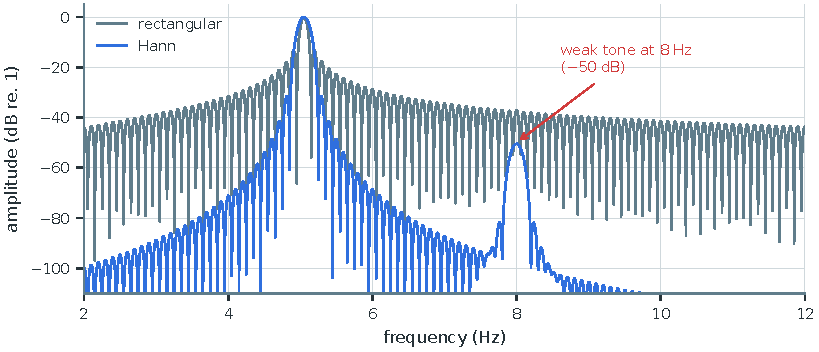
\includegraphics[width=\linewidth]{theory-window-leakage}
\caption{Leakage. Spectrum of a tone at 5.05~Hz (not on a bin) plus a tone 50~dB weaker at 8~Hz, $N=1000$ samples at
100~Hz. The Hann window (blue) reveals the weak tone that the rectangular window (grey) hides.}\label{fig:leak}
\end{figure}

\Cref{tab:windows} gives the measured properties of the three windows used by the application. They were computed
numerically for $N=1024$ with a zero-padded transform.

\begin{table}[tbp]
\centering\small
\caption{Properties of the windows used in RS3D. $\sum w/N$ is the coherent gain; ENBW (equivalent noise bandwidth)
and the null-to-null main-lobe width are in bins; the peak sidelobe is relative to the peak.}\label{tab:windows}
\setlength{\tabcolsep}{4pt}\begin{tabular}{@{}lccccl@{}}
\toprule
Window & $\sum w / N$ & ENBW & Main lobe & Sidelobe (dB) & Used for \\ \midrule
Rectangular & 1.000 & 1.000 & 2.0 & −13.3 & (no taper) \\
Hann & 0.500 & 1.501 & 4.0 & −31.5 & amplitude spectrum \\
Tukey, $\alpha = 0.25$ & 0.875 & 1.102 & 2.3 & −13.6 & spectrogram \\
\bottomrule
\end{tabular}

\end{table}

\section{Scaling the amplitude spectrum}
Raw DFT values grow with $N$ and are changed by the window, so they are not directly interpretable. The
application scales the spectrum so that a sinusoid of amplitude $A$ reads $A$. For
$x[n]=A\cos(2\pi f_0 n/\fs)$ with $f_0$ at the centre of bin $k_0$, and a window $w[n]$, a short calculation
(Appendix~\ref{app:scale}) gives
\begin{equation}\label{eq:ampscale}
  \abs{X_w[k_0]} \;=\; \frac{A}{2}\sum_{n} w[n]
  \quad\Longrightarrow\quad
  A \;=\; \frac{2\,\abs{X_w[k_0]}}{\sum_n w[n]} .
\end{equation}
The amplitude spectrum is therefore
\begin{equation}\label{eq:ampspec}
  A[k] = \frac{2\,\abs{X_w[k]}}{\sum_n w[n]},
\end{equation}
which is in the units of the signal (counts, or m/s). The factor 2 accounts for the energy that the one-sided
spectrum folds in from negative frequencies.
Equation~\eqref{eq:ampscale} assumes the tone lies on a bin centre. A tone that falls midway between two bins
reads low by the window's \emph{scalloping loss}, about 1.4~dB (15\,\%) for the Hann window.

\begin{rs3dapp}
\code{amplitude\_spectrum} (\file{core/spectro.py}) computes exactly~\eqref{eq:ampspec} with the \textbf{Hann}
window~\eqref{eq:hann}: it subtracts the mean of the \emph{valid} samples, multiplies by the window, takes the real
FFT, scales by $2/\sum w$, and discards the zero-frequency bin so that a logarithmic frequency axis is possible. A
window with fewer than 8 valid samples returns empty arrays.

\emph{Gaps.} Samples that are masked or not finite are set to zero after the mean is removed, and the scale uses the
sum of the window over the \emph{valid} samples only, $\sum_{n\in\text{valid}} w[n]$. With this rule a tone keeps its true
amplitude even when part of the window is missing (\cref{fig:ampscale}); without it, the hidden fill values of an
integer trace would dominate the spectrum.
\end{rs3dapp}

\begin{figure}[tbp]
\centering
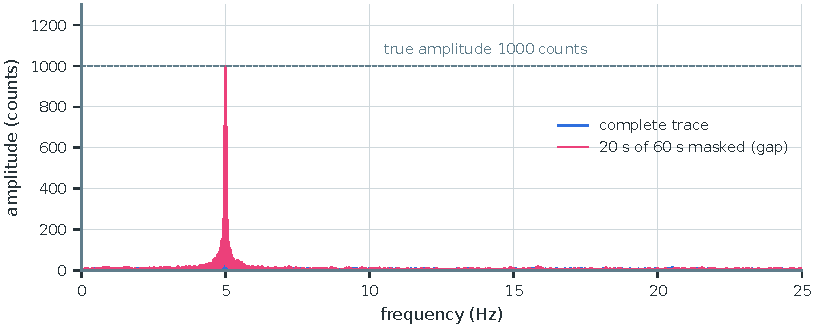
\includegraphics[width=\linewidth]{theory-amplitude-scaling}
\caption{Output of the application's \code{amplitude\_spectrum} for a 5~Hz sine of amplitude 1000~counts in noise,
with the trace complete (blue) and with 20~s of 60~s masked (pink). Both peak at 1000~counts.}\label{fig:ampscale}
\end{figure}

\section{Amplitude spectrum versus power spectral density}
An amplitude spectrum suits \emph{deterministic} signals such as tones, whose amplitude is meaningful. For
\emph{random} signals such as ground noise the meaningful quantity is the one-sided power spectral density (PSD),
the power per unit frequency. For a window $w$ the periodogram estimate is
\begin{equation}\label{eq:psd}
  S_{xx}[k] = \frac{2\,\abs{X_w[k]}^{2}}{\fs\sum_n w[n]^{2}}
  \qquad(\text{counts}^{2}/\text{Hz}),
\end{equation}
which integrates over frequency to the variance of the signal. The two are related, for a tone, by
$S_{xx}\,B_{\mathrm{ENBW}} = A^{2}/2$, where $B_{\mathrm{ENBW}}=\mathrm{ENBW}\cdot\df$ is the equivalent noise bandwidth in hertz. The Spectra mode shows amplitude; the spectrogram and the noise
spectrum (Chapters~\ref{ch:spectrogram} and~\ref{ch:noise}) show PSD in decibels.

\section{Variance of a spectrum estimate and why averaging helps}
The DFT of a random signal is itself random. For Gaussian noise the periodogram~\eqref{eq:psd} at a given frequency
is proportional to a $\chi^{2}$ variable with two degrees of freedom, whose standard deviation equals its mean:
the estimate does not become more reliable by making $N$ larger, it only becomes finer. This is the jagged look of a
single-window spectrum in \cref{fig:noisespec}.

\textcite{welch1967} reduced the variance by dividing the record into $K$ (possibly overlapping) segments,
computing a windowed periodogram of each, and averaging: the variance falls roughly as $1/K$ at the price of
resolution $K$ times coarser than the whole record would allow. The smooth blue curve in \cref{fig:noisespec} is the
root-mean-square average of 24 two-minute windows of the same night-time noise.

\begin{figure}[tbp]
\centering
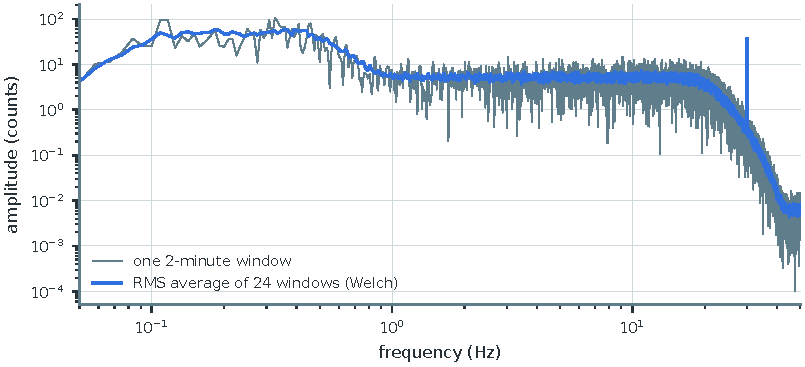
\includegraphics[width=\linewidth]{theory-noise-spectrum}
\caption{Amplitude spectrum of the night-time demo noise (EHZ, from 02:00~UTC). A single two-minute window (grey) is
jagged; the RMS average of 24 consecutive windows (blue) is smooth. The narrow line at 30~Hz is a deliberate
instrument line in the demo data.}\label{fig:noisespec}
\end{figure}

\begin{rs3dkey}
An amplitude spectrum is exact for tones and scaled by $2/\sum w$; a single-window spectrum of noise is always
jagged, and only averaging, as the spectrogram and noise spectrum do, makes it reliable.
\end{rs3dkey}
